%! Licence = CC BY-NC-SA 4.0

%! Author = gianfluetsch
%! Date = 22. Jan 2022
%! Project = icth_summary

\section{Signale}
\subsection{Rinkel}
\subsubsection{FS2015}
Sie planen einen Subwoofer zu bauen und wissen, dass die minimale Phasenverschie-bung zwischen dem linken und rechten Ohr, die ein Mensch zur Lokalisierung der Schallquelle noch auswerten kann bei 0.2 rad liegt.
Bestimmen sie die obere Grenzfrequenz, die der Subwoofer maximal abgeben darf.\\

Gehen sie dabei von den folgenden Annahmen aus. Der Abstand von einem Ohr zum anderen ist  im Mittel mit 21 cm gegeben. Die Schallgeschwindigkeit wird mit 330 m/s angenommen.\\

Stellen sie die maximale Phasenverschiebung des Audiosignals von einem zum anderen Ohr als Funktion der Frequenz dar.\\

$\phi(f)=2\pi f s/v = f = \frac{\phi}{2\pi}*\frac{s}{v}$\\
$f=\frac{0.2*330 m/s}{2\pi*0.21m} = 50 Hz$\\

Fourier:  Gegeben ist ein Generator der folgendes Dreieckssignal mit der Frequenz von 3 kHz generiert:
\begin{center}
    \vspace{-8pt}
    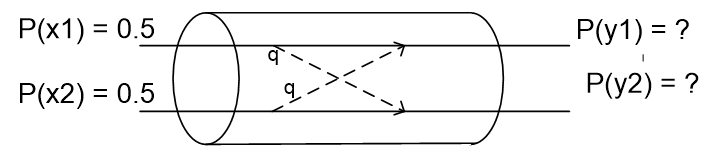
\includegraphics[width=.6\linewidth]{./03-signale/fs2015}
    \vspace{-8pt}
\end{center}

Sie wollen ein harmonisches Signal mit der Frequenz von 9 kHz erzeugen. Entwickeln Sie eine Prinzipschaltung unter Angabe aller signifikanten Werte, die dies realisiert.\\
$y(t)=\frac{8\hat{y}}{\pi^2}(\frac{1}{1^2}*sin(\omega_0 t)-\frac{1}{3^2}*sin(3\omega_0 t)+\frac{1}{5^2}*sin(5\omega_0 t)-...)$\\
\textit{Die Frequenz von 9 kHz entspricht der zweiten harmonischen $\rightarrow$ durch einen Bandpass mit der unteren Grezfrequenz von z.B. 8 khz und einer oberen Grenzfrequenz von z. Bsp 10 kHz }\\

Wie gross ist die Amplitude dieser harmonischen Schwingung?\\
$a=\frac{8*10V}{9*\pi^2}=0.9V$\\

Um wie viel db ist dann das Ausgangssignal gegenüber dem Eingangssignal gedämpft?\\
$a=10log\frac{0.9V}{10V}=-10.46db$\\

Wie hoch ist dann der Pegel in V beim Empfänger, wenn die nachgeschaltete Übertra-gungsstrecke eine Dämpfung von 3 db aufweist?\\
$-13.46db = 10log\frac{x}{10}$\\
$10^{-1.346}*10V = 0.045V$

\subsubsection{Prüfung HS2009}
Zur Verschleierung von Sprachsignalen wird das System in Bild unten, auch Scrambler genannt, eingesetzt. Es transformiert das Signalspektrum in die Kehrlage und wurde beispielweise im Mobilfunknetz C eingesetzt.\\
\begin{center}
    \vspace{-8pt}
    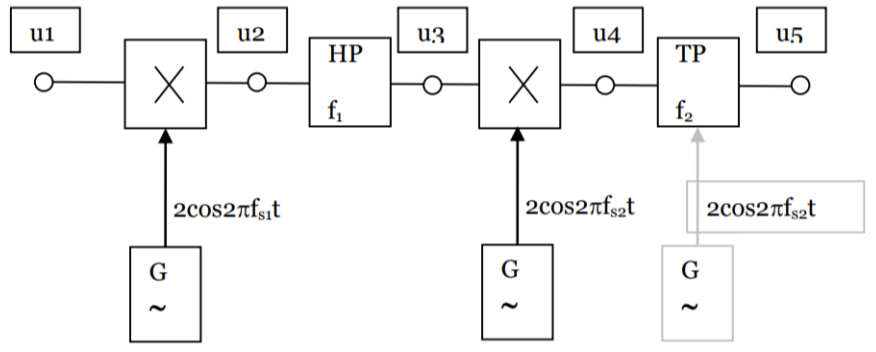
\includegraphics[width=.6\linewidth]{./03-signale/hs2009_6}
    \vspace{-8pt}
\end{center}

Was versteht man unter Kehrlage eines Signals?\\
\textit{Das höherfrequente Nachchtensignal liegt in beiden Seitenbändern näher bei der Trägerfrequenz als das niedfrequente Nachrichtensignal.}\\

Analysieren Sie das System, indem Sie die Spektren der Signale u1 bis u5 skizzieren. Es ist g die Grenzfrequenz des Eingangssignals u1.\\
Geben Sie ferner die Frequenzen f1, f2 sowie fs1 und fs2 zueinander so an, dass der Scrambler seine Aufgabe erfüllen kann.
\begin{center}
    \vspace{-8pt}
    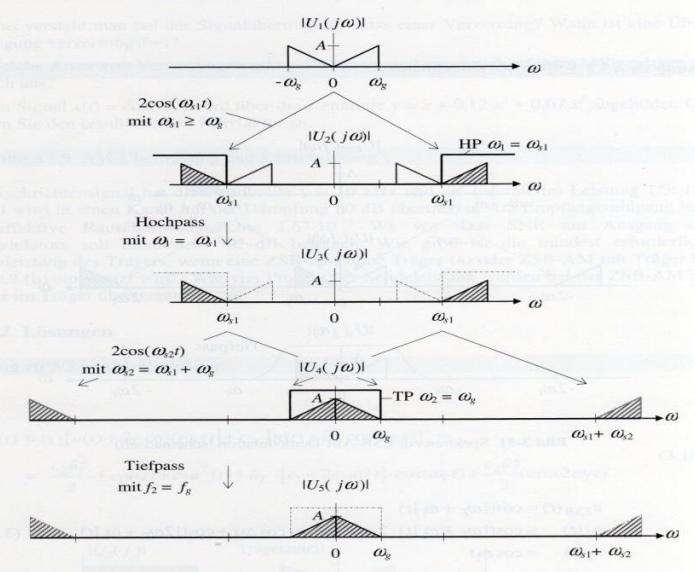
\includegraphics[width=.6\linewidth]{./03-signale/hs2009_7}
    \vspace{-8pt}
\end{center}

Gegeben ist das folgende Spektrum eines modulierten Sprachsignals.
\begin{center}
    \vspace{-8pt}
    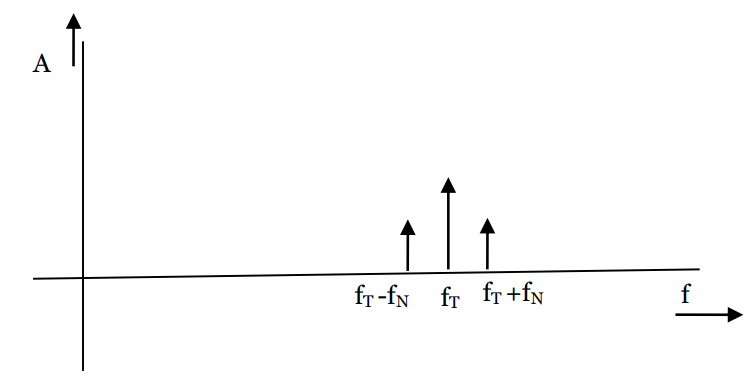
\includegraphics[width=.6\linewidth]{./03-signale/hs2009_8}
    \vspace{-8pt}
\end{center}

Befindet sich das Sprachsignal fN in der Kehr- oder Regellage? (Anm. die Frequenz fN ist die obere Grenzfrequenz des Sprachsignals)\\
\textit{Das Signal befindet sich nicht in der Kehrlage.}\\

Konstruieren Sie eine Demodulatoschaltung und zeigen sie rechnerisch, dass das Sprachsignal fN im Basisband vorliegt.\\
\begin{center}
    \vspace{-8pt}
    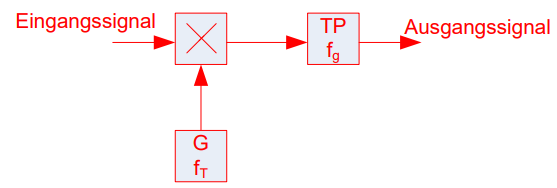
\includegraphics[width=.6\linewidth]{./03-signale/hs2009_9}
    \vspace{-8pt}
\end{center}

\begin{center}
    \vspace{-8pt}
    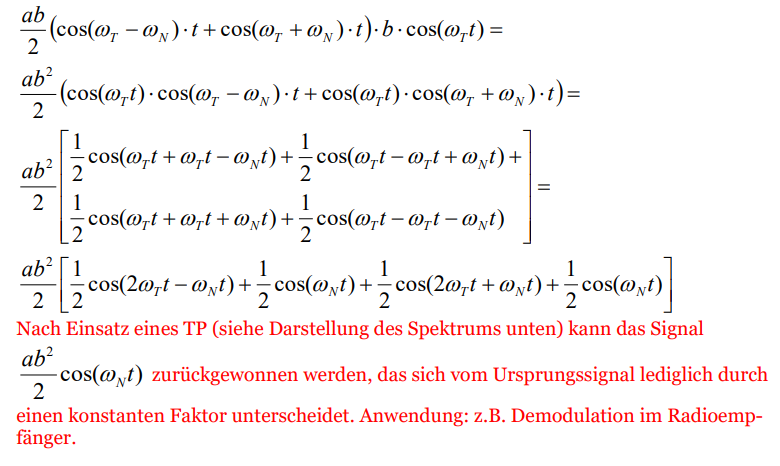
\includegraphics[width=.8\linewidth]{./03-signale/hs2009_10}
    \vspace{-8pt}
\end{center}

\subsubsection{Prüfung FS2009}
Gegeben ist das folgende Blockschaltbild:
\begin{center}
    \vspace{-8pt}
    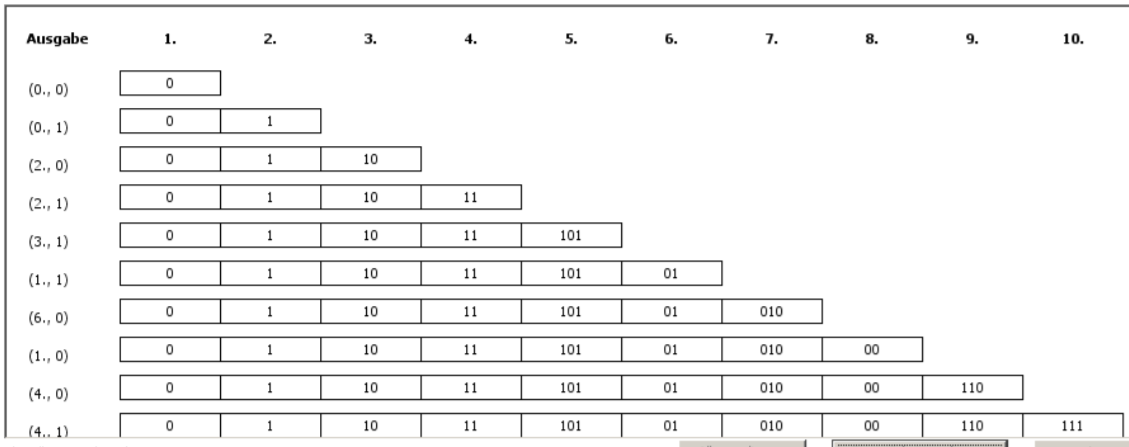
\includegraphics[width=.8\linewidth]{./03-signale/fs2009}
    \vspace{-8pt}
\end{center}

Zeichnen Sie das Frequenzspektrum, das Sie an dem Punkt1, dem Punkt 2 und dem Punkt 3 beobachten können.\\
\textit{Die Fourierzerlegung folgt für}\\
$f(x)=a(sin(x)+\frac{sin(2x)}{2}+\frac{sin(3x)}{3}+...)$\\

\textit{Das positive Sägezahnsignal zu:}\\
$f(x)=a(\frac{1}{1^2}*sin(x)-\frac{sin(3x)}{3^2}+\frac{sin(5x)}{5^2}-....)$\\

\textit{Und das Dreieckssignal zu:}
\begin{center}
    \vspace{-8pt}
    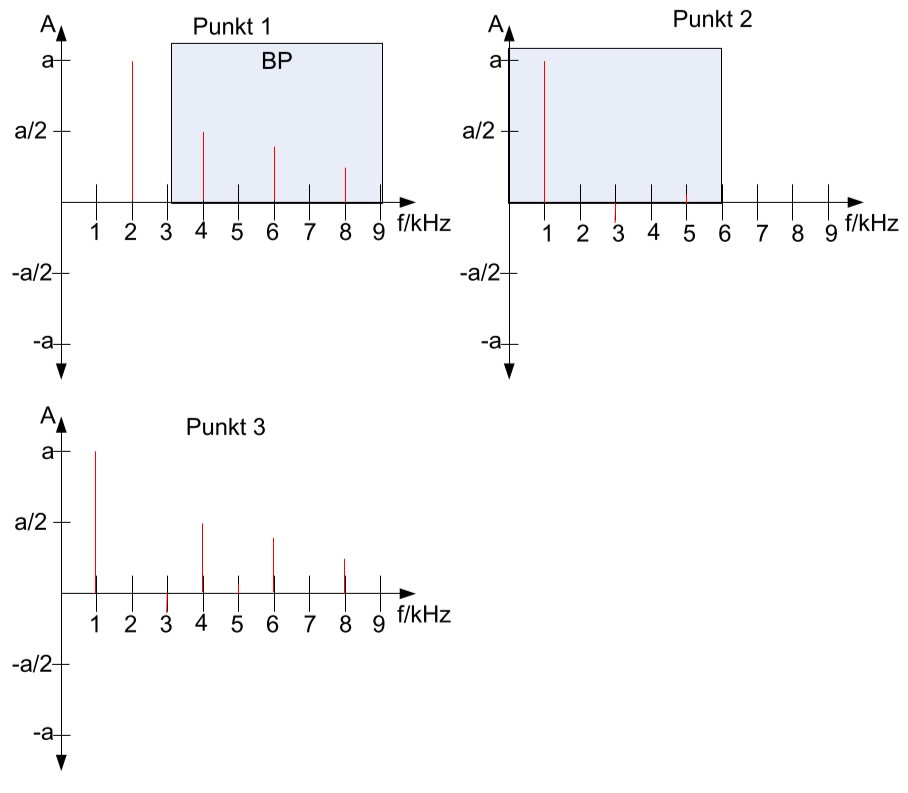
\includegraphics[width=.8\linewidth]{./03-signale/fs2009_2}
    \vspace{-8pt}
\end{center}



